\documentclass[tikz,border=8pt]{standalone}
% Shared look for every TikZ diagram. Load with % Shared look for every TikZ diagram. Load with % Shared look for every TikZ diagram. Load with \input{../../tools/tikz-style.tex}
\usepackage[T1]{fontenc}
\usepackage{lmodern}
\renewcommand{\sfdefault}{lmr}  % diagrams use the same serif as the text
\usetikzlibrary{arrows.meta, positioning, shapes.geometric, calc, fit, backgrounds}
\definecolor{cblue}{HTML}{4C78A8}
\definecolor{corange}{HTML}{F58518}
\definecolor{cgreen}{HTML}{54A24B}
\definecolor{cred}{HTML}{E45756}
\definecolor{cpurple}{HTML}{B279A2}
\definecolor{cgrey}{HTML}{6B6B6B}
\tikzset{
  every picture/.style={font=\sffamily, line width=1.2pt},
  box/.style={draw=#1, fill=#1!12, rounded corners=4pt, align=center, inner sep=7pt, minimum height=1.1cm},
  box/.default=cgrey,
  arrow/.style={-{Stealth[length=3mm]}, draw=cgrey, line width=1.4pt},
  title/.style={font=\sffamily\bfseries\Large},
  note/.style={font=\sffamily\small, text=cgrey, align=center},
}
\AtBeginDocument{\hyphenpenalty=10000 \exhyphenpenalty=10000}

\usepackage[T1]{fontenc}
\usepackage{lmodern}
\renewcommand{\sfdefault}{lmr}  % diagrams use the same serif as the text
\usetikzlibrary{arrows.meta, positioning, shapes.geometric, calc, fit, backgrounds}
\definecolor{cblue}{HTML}{4C78A8}
\definecolor{corange}{HTML}{F58518}
\definecolor{cgreen}{HTML}{54A24B}
\definecolor{cred}{HTML}{E45756}
\definecolor{cpurple}{HTML}{B279A2}
\definecolor{cgrey}{HTML}{6B6B6B}
\tikzset{
  every picture/.style={font=\sffamily, line width=1.2pt},
  box/.style={draw=#1, fill=#1!12, rounded corners=4pt, align=center, inner sep=7pt, minimum height=1.1cm},
  box/.default=cgrey,
  arrow/.style={-{Stealth[length=3mm]}, draw=cgrey, line width=1.4pt},
  title/.style={font=\sffamily\bfseries\Large},
  note/.style={font=\sffamily\small, text=cgrey, align=center},
}
\AtBeginDocument{\hyphenpenalty=10000 \exhyphenpenalty=10000}

\usepackage[T1]{fontenc}
\usepackage{lmodern}
\renewcommand{\sfdefault}{lmr}  % diagrams use the same serif as the text
\usetikzlibrary{arrows.meta, positioning, shapes.geometric, calc, fit, backgrounds}
\definecolor{cblue}{HTML}{4C78A8}
\definecolor{corange}{HTML}{F58518}
\definecolor{cgreen}{HTML}{54A24B}
\definecolor{cred}{HTML}{E45756}
\definecolor{cpurple}{HTML}{B279A2}
\definecolor{cgrey}{HTML}{6B6B6B}
\tikzset{
  every picture/.style={font=\sffamily, line width=1.2pt},
  box/.style={draw=#1, fill=#1!12, rounded corners=4pt, align=center, inner sep=7pt, minimum height=1.1cm},
  box/.default=cgrey,
  arrow/.style={-{Stealth[length=3mm]}, draw=cgrey, line width=1.4pt},
  title/.style={font=\sffamily\bfseries\Large},
  note/.style={font=\sffamily\small, text=cgrey, align=center},
}
\AtBeginDocument{\hyphenpenalty=10000 \exhyphenpenalty=10000}

% Section 6: student 1 through the classification network. Each node: weighted sum z, then sigmoid.
% z = 1.6 -> 0.832 (hidden), z_f = 0.166 -> 0.5415 (output), L = -log 0.5415 = 0.613.
\begin{document}
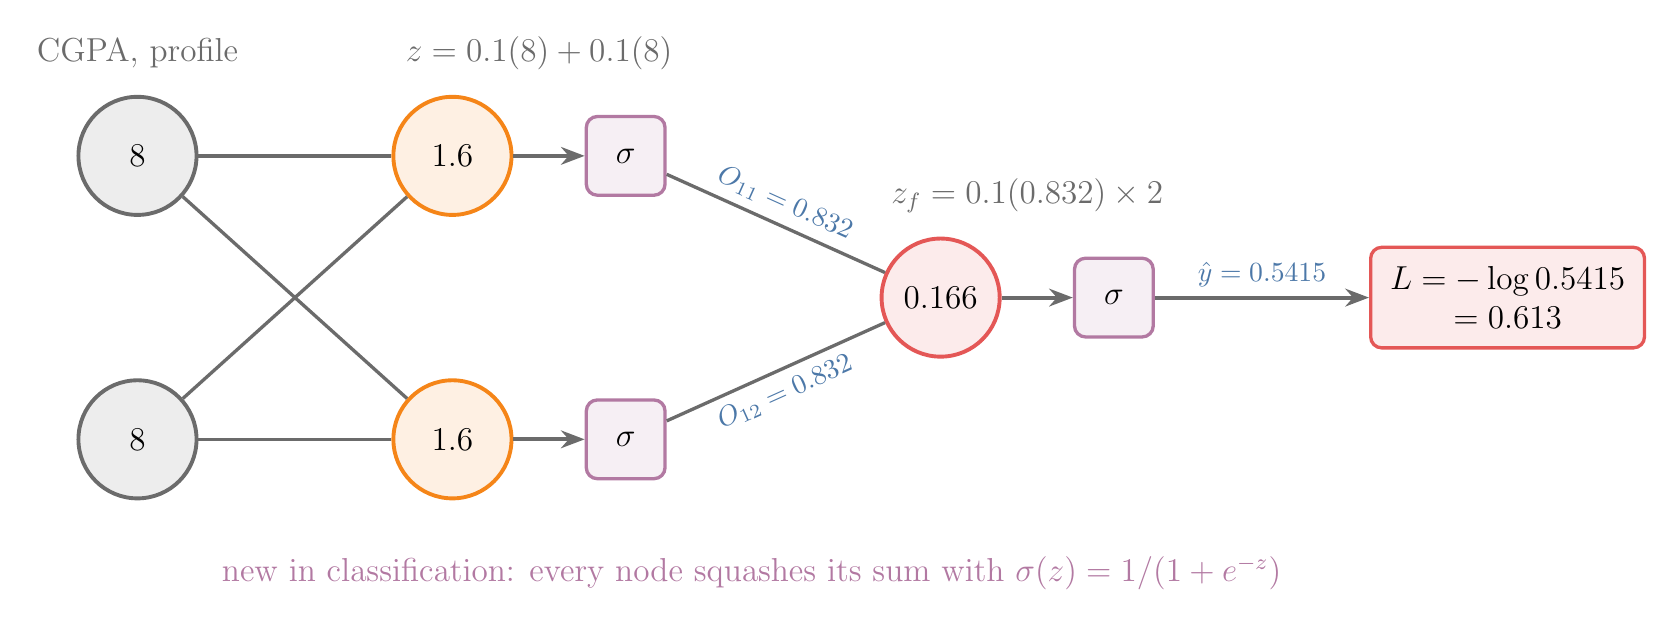
\begin{tikzpicture}[n/.style={circle, draw=#1, fill=#1!12, minimum size=1.5cm, font=\large, line width=1.4pt},
                    sig/.style={box=cpurple, minimum width=1.0cm, minimum height=1.0cm, font=\large, inner sep=3pt},
                    v/.style={font=\normalsize, text=cblue},
                    e/.style={draw=cgrey, line width=1.2pt}]
  \node[n=cgrey] (x1) at (0, 1.8) {8};
  \node[n=cgrey] (x2) at (0, -1.8) {8};
  \node[n=corange] (z1) at (4, 1.8) {$1.6$};
  \node[n=corange] (z2) at (4, -1.8) {$1.6$};
  \node[sig] (s1) at (6.2, 1.8) {$\sigma$};
  \node[sig] (s2) at (6.2, -1.8) {$\sigma$};
  \node[n=cred] (zf) at (10.2, 0) {$0.166$};
  \node[sig] (sf) at (12.4, 0) {$\sigma$};
  \node[box=cred, font=\large] (L) at (17.4, 0) {$L = -\log 0.5415$\\$= 0.613$};
  \foreach \a in {x1, x2} \foreach \b in {z1, z2} \draw[e] (\a) -- (\b);
  \draw[arrow] (z1) -- (s1); \draw[arrow] (z2) -- (s2);
  \draw[e] (s1) -- node[v, above, sloped] {$O_{11} = 0.832$} (zf);
  \draw[e] (s2) -- node[v, below, sloped] {$O_{12} = 0.832$} (zf);
  \draw[arrow] (zf) -- (sf);
  \draw[arrow] (sf) -- node[v, above] {$\hat y = 0.5415$} (L);
  \node[note, font=\large] at (0, 3.1) {CGPA, profile};
  \node[note, font=\large] at (5.1, 3.1) {$z = 0.1(8) + 0.1(8)$};
  \node[note, font=\large] at (11.3, 1.3) {$z_f = 0.1(0.832) \times 2$};
  \node[note, font=\large, text=cpurple] at (7.8, -3.5) {new in classification: every node squashes its sum with $\sigma(z) = 1/(1 + e^{-z})$};
\end{tikzpicture}
\end{document}
